\documentclass[11pt]{standalone}
\usepackage{amssymb}
\usepackage{amsmath}
\usepackage[no-math]{fontspec}
\usepackage{unicode-math}
\usepackage{libertinus}
\usepackage{pgf,xcolor}
\usepackage{tikz}
\usetikzlibrary{arrows.meta, backgrounds}
\usepackage{pgfplots}
\pgfplotsset{compat=newest}

\definecolor{my_darkgray}{HTML}{484949}
\definecolor{my_lightgray}{HTML}{F3F4F4}
\definecolor{my_darkblue}{HTML}{005A94}
\definecolor{my_lightblue}{HTML}{CCDEE9}
\definecolor{my_yellow}{HTML}{FFEC7F}
\definecolor{my_red}{HTML}{E60000}
\definecolor{my_orange}{HTML}{E87846}

\begin{document}
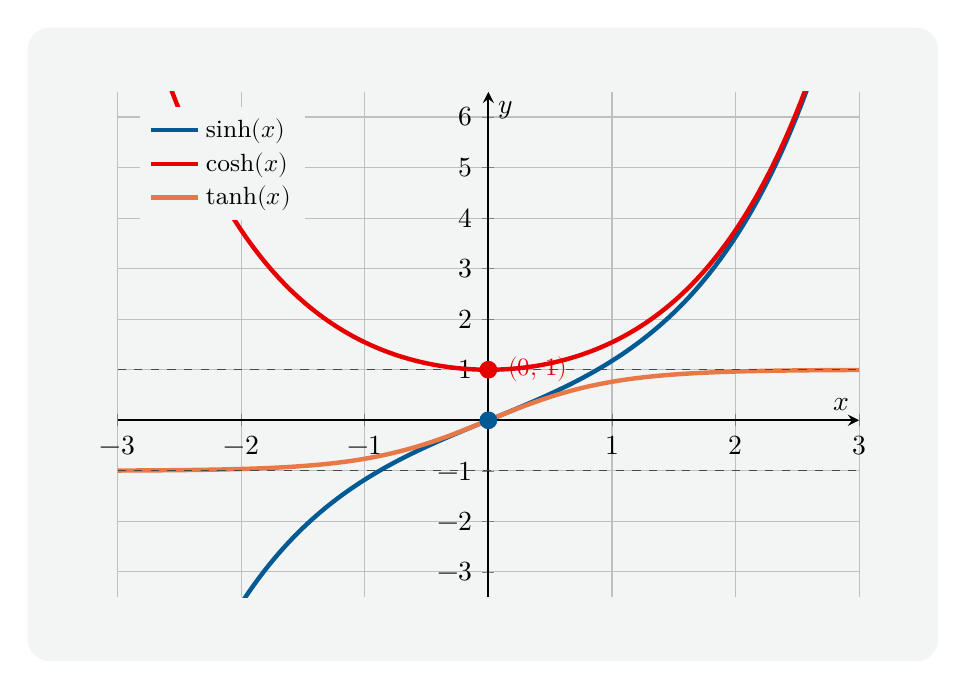
\begin{tikzpicture}[
    show background rectangle,
    background rectangle/.style={fill=my_lightgray, rounded corners=8pt},
    inner frame sep=0.8cm
]
\begin{axis}[
    axis lines=center,
    xlabel={$x$},
    ylabel={$y$},
    height=8cm, width=11cm,
    xmin=-3.0, xmax=3.0,
    ymin=-3.5, ymax=6.5,
    xtick={-3,-2,-1,0,1,2,3},
    ytick={-3,-2,-1,0,1,2,3,4,5,6},
    grid=both,
    axis line style={thick},
    restrict y to domain=-4:7,
    clip=true,
    legend style={
        font=\small,
        at={(0.03, 0.97)},
        anchor=north west,
        draw=none,
        fill=my_lightgray,
    },
    legend cell align=left,
]

% sinh(x) = (e^x - e^{-x})/2  — odd function, passes through origin
% (my_darkblue): primary curve
\addplot[draw=my_darkblue, samples=300, ultra thick, domain=-3:3]
    {(exp(x) - exp(-x))/2};
\addlegendentry{$\sinh(x)$}

% cosh(x) = (e^x + e^{-x})/2  — even function, minimum 1 at x=0
% (my_red): secondary curve
\addplot[draw=my_red, samples=300, ultra thick, domain=-3:3]
    {(exp(x) + exp(-x))/2};
\addlegendentry{$\cosh(x)$}

% tanh(x) = sinh(x)/cosh(x)  — odd, bounded in (-1, 1)
% (my_orange): tertiary curve
% Note: the section caption calls this curve "green" but the palette has no
% green; my_orange is used as the third curve color per the style guide.
\addplot[draw=my_orange, samples=300, ultra thick, domain=-3:3]
    {(exp(x) - exp(-x))/(exp(x) + exp(-x))};
\addlegendentry{$\tanh(x)$}

% Horizontal asymptotes of tanh at y = ±1 (dashed, my_darkgray)
\addplot[draw=my_darkgray, dashed, thin, domain=-3:3]{ 1};
\addplot[draw=my_darkgray, dashed, thin, domain=-3:3]{-1};

% Mark the minimum of cosh at (0, 1)
\addplot[only marks, mark=*, mark size=3pt, draw=my_red, fill=my_red]
    coordinates{(0, 1)};
\node[right, font=\small, my_red] at (axis cs:0.08, 1) {$(0,\,1)$};

% Mark the zero of sinh and tanh at the origin
\addplot[only marks, mark=*, mark size=3pt, draw=my_darkblue, fill=my_darkblue]
    coordinates{(0, 0)};

\end{axis}
\end{tikzpicture}
\end{document}
